\documentclass[a4paper,10pt]{article}
%ArXiv allows 10pt - 14pt

\usepackage{publication}
\usepackage[backend=biber, sorting=none]{biblatex}
\addbibresource{references.bib}

\usepackage{siunitx}
\usepackage{amsmath}
\usepackage{amsfonts}

\usepackage{bbold}
\usepackage{csquotes}
\usepackage{graphicx, float}

%Adds the draft watermark
\isdraft

% Title formatting
\title{Stronghold Location via Triangulation and Error Estimation}

\author{PixelRayn}
\contact{@physikdavid}

\keywords{Minecraft, Speedrunning, Tools, Navigation}
\date{\today}

\begin{document}

\maketitle

% Abstract with justification
%\begin{abstract}
%\end{abstract}

%Use this when not including an abstract to print horizontal rule and keywords.
%\noabstract

%Use either of these  to only print the keywords
%\putkeywords                                       %Prints keywords with the vertical margins and the "Keywords" identifier
%\keywordlist                                       %Provides the keywords directly

% Double-column layout
\begin{multicols}{2}

    \section{Introduction}
    Every Minecraft world has a total of 128 strongholds aranged in concentric rings around the origin of the coordinate system \cite{wiki_stronghold}.
    The intended way for a player to locate the closest stronghold is via the eye of ender item.
    When activated the eye of ender flies approximately 12 blocks in the direction of the north-west corner of the chunk containing the spiral staircase room of the stronghold.
    While the eye of ender targets the chunk coordinates (0, 0), the entrance to the stronghold is always generated at coordinates (4, 4).
    When the player is more than 12 blocks from the target coordinate the eye of ender travels upward giving a clear indication of the direction to travel in \cite{wiki_endereye}.

    Since the eye of ender has a $20\unit{\%}$ chance of shattering, which consumes the item, a strategy to minimize the number of pearls thrown is desirable.
    This paper reiterates the algebraic method for locating a stronghold with as little as two eyes of ender and introduced monte carlo simulations to estimate the uncertainty of the calculated location.
    The triangulation method discussed here is not new, instead it has been repeated and passed down through the community so long that the original authorship is now unclear.
    References \cite{tutorial_goosen} and \cite{tutorial_ben} date the methods to at least 2013.

    \section{Triangulation}
    The location of the stronghold in the X-Z plane is calculated using two consecutaive throws of an eyes of ender.
    For each throw the coordinate of the player is noted with the angle of the eyes trajectory via the debug screen \cite{wiki_debugscreen}.
    A large separation of the two location improves accuracy of the estimate.
    Let the target coordinates be
    \begin{equation}
        \vec{r}_t = \begin{bmatrix}
            x_t\\z_t
        \end{bmatrix}
    \end{equation}
    The intersecting headings are parameterized in the X-Z plane by
    \begin{equation}
        f_i(x) = m_i x - z_i^0
    \end{equation}
    Fulfilling the necesarry requirement that
    \begin{equation}
        f_i(x_i) = m_i x_i - z_i^0 = z_i \implies z_i^0 = m_i x_i - z_i
    \end{equation}
    By facing the eye of ender in the air, the yaw direction shown in the debug screen directly corresponds to the travel direction of the eye of ender constraining the target coordinates.
    
    \subsection{Calculating the Line Slope from Yaw}

    The yaw-angle $\theta$ is measured from the z-Axis.
    The south direction (towards positive z) corresponds to $\theta = 0$ and the clockwise direction corresponds to positive angle.
    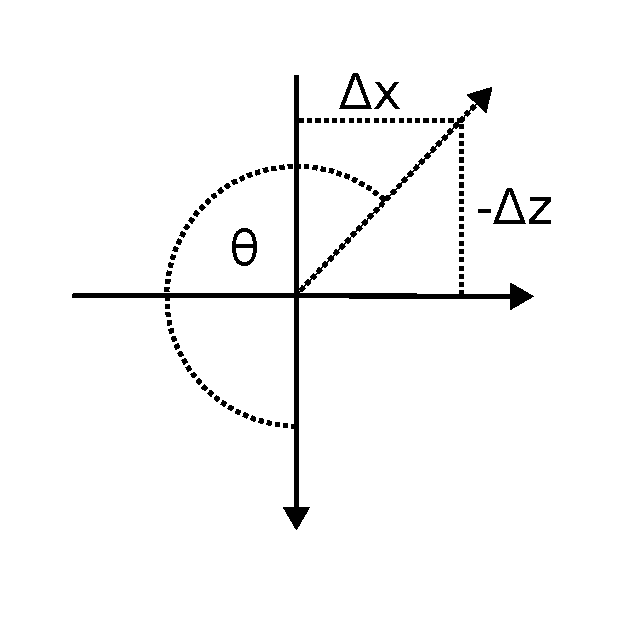
\includegraphics[width = \linewidth]{img/theta.pdf}

    The slope $m$ is calculated as
    \begin{equation}
        m = \frac{\Delta z}{\Delta x} = -\tan(90-\theta)
    \end{equation}

    \subsection{Solving for $\vec r_t$}

    For the two measurement locations two separate functions $f_1$ and $f_2$ are constructed. For $\vec r_t$ the two functions must intersect:
    \begin{equation}
        f_1(x_t) = f_2(x_t) = z_t\\
    \end{equation}
    By explicitly writing the functions as a system of linear equations in respect to $z_t$ and isolating all target terms on the left side of the equation the following can be shown:
    \begin{align}
        m_1 x_t - z_t &= m_1 x_1 - z_1\\
        m_2 x_t - z_t &= m_2 x_2 - z_2
    \end{align}
    The system of linear equations is expressed as:
    \begin{equation}
        \underbrace{
        \begin{bmatrix}
            m_1 & -1\\
            m_2 & -1\\
        \end{bmatrix}}_M
        \cdot
        \underbrace{
        \begin{bmatrix}
            x_t \\ z_t
        \end{bmatrix}}_{\vec r_t}
         =
         \underbrace{
         \begin{bmatrix}
            m_1 x_1 - z_1\\
            m_2 x_2 - z_2\\  
         \end{bmatrix}}_{\vec z_0}
    \end{equation}
    Assuming $m_1 \ne m_2$ and $m_1 \ne -m_2$ M is invertible.
    Since $M^{-1}M = \mathbb{1}$ the calculation of $\vec{r}_t$ is therefore rephrased as inverting the Matrix $M$.

    \begin{equation}
        \vec r_t = M^{-1}{\vec z_0}
    \end{equation}

    One procedure for matrix inversion is the Gauss-Jordan algorithm \cite[436]{alma991016822109706467} which yields the following inverse matrix:

    \begin{equation}
        M^{-1} = \begin{bmatrix}
            \frac{1}{m_1 - m_2} & \frac{1}{m_2 - m_1}\\
            -\frac{m_2}{m_1+m_2} & 1-\frac{m_1}{m_1+m_2}
        \end{bmatrix}
    \end{equation}

    \section{Error Estimation}

    A Monte Carlo simulation-method commonly known as a \enquote{parametric bootstrap} is used to compute the confidence statistics of the estimate \cite[53-56]{efron_1994_introductiontothebootstap}.
    The errors from $x$, $z$, and $\theta$ measurements are assumend to be normally distributed and uncorrelated. Samples are drawn from the simulated probability density functions and the predicted stronghold position is calculated for each simulated measurement.
    Confidence intervals are chosen at the upper and lower quantile to correspond to a $1\sigma$ interval for $x$ and $z$ independently.
    Drawing a histogram for an example set of measurements reveals a strong correlation between the $x$ and the $z$ coordinate for measurements with little angular separation as an emergent property of the measurement. (Compare fig. \ref{fig:histo}.) 

    \begin{figure}[H]
        \centering
        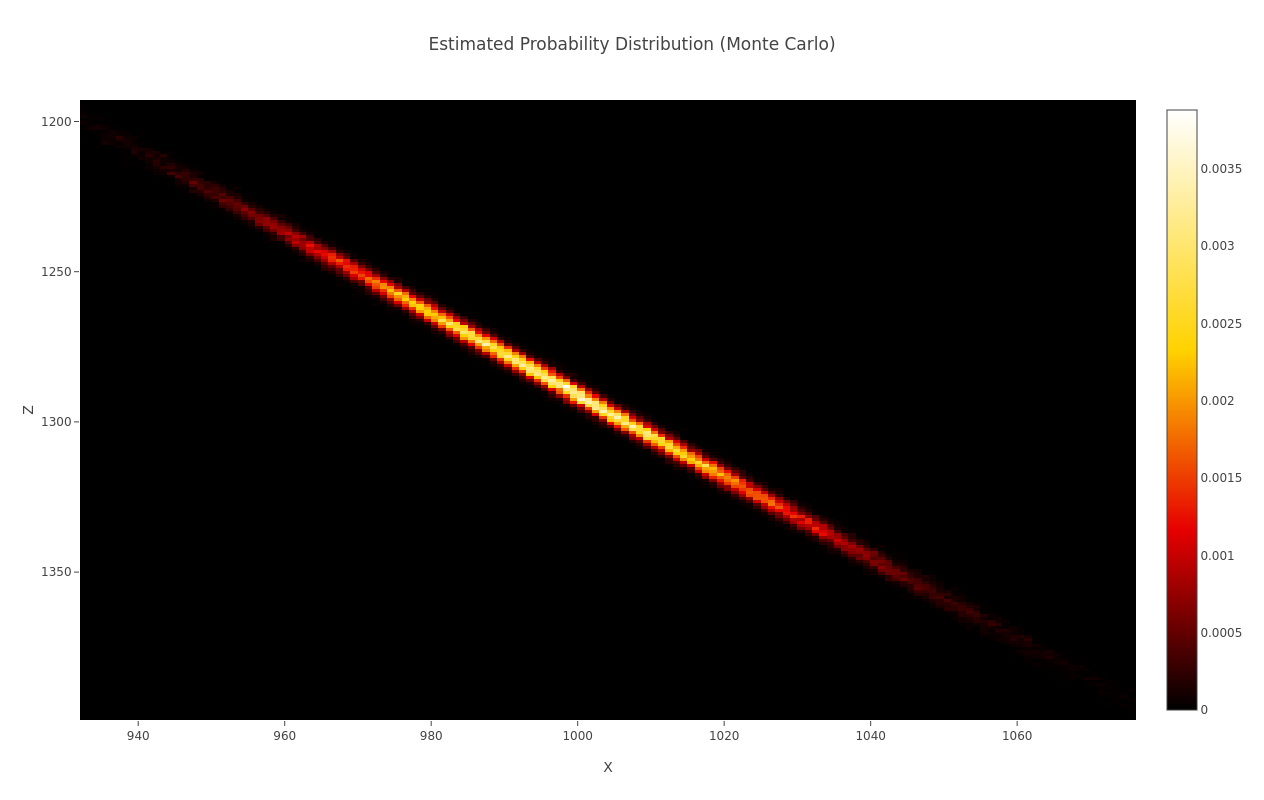
\includegraphics[width = \linewidth]{img/distribution_large.png}
        \caption{Example measurement of a stronghold position with $x_1 = 10$, $z_1 = 33$, $\theta_1 = -38.2\unit{\degree}$, $x_2 = 119$, $z_2 = 19$, $\theta_2 = -34.7\unit\degree$. Errors are estimated with $\Delta x = \Delta z = 0.5$ and $\Delta \theta = 0.1\unit\degree$. Graphic is generated with Ref. \cite{repo_triang}}
        \label{fig:histo}
    \end{figure}

    \section{Conclusion}

    A method for triangulating the stronghold location is formally reintroduced and a numeric method for estimating the uncertainties is discussed. A localy running implementation using JavaScript can be found in ref. \cite{repo_triang}.
\end{multicols}

\printbibliography


\end{document}
